% !Tex root = thesis.tex

% Appendices
\appendix \label{apdx}

%\chapter{Glossary of Notation}
%abc


\chapter{Artificial Neural Networks} \label{apdx:ann}
Artificial Neural Networks (ANN) are commonly understood to be complicated black box machine learning methods which produce high levels of accuracy, while sacrificing interpretability \cite{pattern_rec_book}. This assessment is true in part -- the end-to-end decision process of a trained neural network is very convoluted. But after zooming in to the inner workings of an ANN, each individual part is quite simple.

\section{Architecture}
Neural networks have a graph-like structure with vertices (nodes) and weighted edges. A basic feed-forward neural network (FFN) consists of an input layer, a number of hidden layers, and an output layer. A ``layer'' $l$ consists of $n_l$ nodes, and each node $i$ is connected to every node in the previous layer $l-1$ by a weighted edge. In this manner, the subgraph containing all nodes of layer $l-1$ and all nodes of layer $l$ can be seen as a complete bipartite graph $K_{n_{l-1}, n_l}$. A simple FFN is shown in Figure \ref{fig:ffn_example} which takes inputs with 10 features and classifies into three categories \cite{nn_svg}. For example, inputs could represent the weight, height, hair length, etc. of a pet, with the task of classifying the pet as a cat, dog, or bird \cite{neural_net}.

\sideremark{Edit this image with correct notation}
\begin{figure}[h]
  \centering
  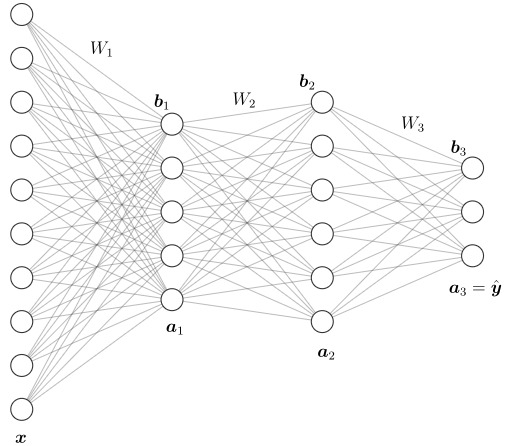
\includegraphics[width=.85\textwidth]{img/ffn_visual.png}
  \caption{A basic FFN with input size $n_0 = 10$ and output size $n_3 = 3$, with two hidden layers of size $n_1 = 5$ and $n_2 = 6$.}
  \label{fig:ffn_example}
\end{figure}

While the architecture of a neural network can be described using the lens of graph theory, the inner workings are better described using basic linear algebra. Each layer acts as a function from $\R^{n_{l-1}}$ to $\R^{n_{l}}$. Specifically, this function is a linear transformation followed by a nonlinear re-scaling. For a given input vector $\vect x^* \in \R^{n_0}$ and its corresponding true label $\vect y^*$, the value in the first hidden layer is calculated as
\begin{equation}
  \vect a_1^* = f_1(W_1 \vect x^* + \vect b_1)
  \label{eq:hid_layer}
\end{equation}
where $W_1 \in \R^{n_1 \times n_0}$ and $\vect b_1 \in\R^{n_1}$ are the trainable \textit{weights} matrix and \textit{bias} vector. The notion of ``trainable'' parameters is explored further in Appendix \ref{apdx:backprop}. The value $\vect a_1^*$ is called the \textit{activation} value of the input $\vect x^*$ at hidden layer $l=1$. The non-decreasing function $f_1$ is called an \textit{activation function} which applies a (possibly) non-linear rescaling to the vector $\vect z_1^* = W_1 \vect x^* + \vect b_1 \in \R^{n_1}$ elementwise. Examples of different activation functions are given in Appendix \ref{apdx:activation_fcns}. Matrix notation can also be abandoned by writing the activation of the $i$-th node in layer $l=1$ as 
\begin{equation}
  a_{1,i}^* = f_1\left(b_{1,i} + \sum_{j=1}^{n_0} w_{ij}^1 \cdot x_j^* \right)
  \label{eq:element_activation}
\end{equation}
where $w_{ij}^1$ is the element in the $i$-th row and $j$-th column of $W_1$, the weight connecting the $j$-th node of layer $0$ to the $i$-th node of layer $1$.

The activation value of the input $\vect x^*$ at hidden layer $l=2$ and the output layer $l=3$ can similarly be computed as
\begin{equation}
  \begin{split}
    \vect a_2^* &= f_2(W_2 \vect a_1^* + \vect b_2) \\
    \hat{\vect y}^* &= \vect a_3^* = f_3(W_3 \vect a_2^* + \vect b_3)
  \end{split}
  \label{eq:ffn_comp}
\end{equation}
where the weights matrices $W_2 \in \R^{n_2 \times n_1}$ and $W_3 \in \R^{n_3 \times n_2}$ and bias vectors $\vect b_2 \in \R^{n_2}$ and $\vect b_3 \in \R^{n_3}$ are trainable. Before training, all trainable parameters are typically initialized randomly. The output value $\hat{\vect y}^*$ serves as the prediction for input $\vect x^*$. 

For classification, the true label is often a one-hot encoding, so the prediction $\hat{\vect y}^*$ should be a probability distribution each entry describes the certainty of model in classifying the input $\vect x^*$ as each possible class. Returning to the earlier example, an input with features pertaining to a cat has the true label $(1,0,0)$. An output prediction may give $(0.65, 0.32, 0.03)$, meaning that the neural network is $65\%$ sure that the input features are that of a cat, $32\%$ sure that the input is a dog, and $3\%$ sure that the input is a bird.

\section{Activation Functions} \label{apdx:activation_fcns}
The main purpose of activation functions is to rescale each layer so that every activation value falls in the same range. Doing multiple matrix multiplications in a row can easily cause values to become very large, and leading to overfitting and other complications \cite{sibi2013}. It can be helpful to use an activation function to map values to the range of $(0,1)$ because of the effect of the numbers $0$ and $1$ in multiplication, map to $(-1,1)$ to utilize positive and negative values, or map to $[0,\infty)$ to avoid negative values. 

Though custom activation functions can be defined and easily implemented, below are a few examples of popular activation functions used in neural networks \cite{tensorflow} \cite{keras_r}. Each of these are applied to a vector elementwise independently, except for the softmax function which maps an $n$-dimensional vector to an $n$-dimensional probability distribution.

\begin{equation}
  \text{Sigmoid: } \sigma(z) = \frac{1}{1 + e^{-z}} \quad \quad \R \to (0,1) 
  \label{eq:sigmoid_eqn}
\end{equation}
The sigmoid activation function has the form of the logistic curve and maps values to be between $0$ and $1$.

\begin{equation}
  \text{Hyperbolic tangent: } \tanh(z) = \frac{e^z - e^{-z}}{e^z + e^{-z}} \quad \quad \R \to (-1,1)
  \label{eq:tanh_eqn}
\end{equation}
Hyperbolic tangent has a similar curvature to that of the sigmoid, but maps values to between $-1$ and $1$. 

\begin{equation}
  \text{Rectified Linear Unit (ReLU): } \text{relu}(z) = \max\{0, z\} \quad \quad \R \to (0,\infty)
  \label{eq:relu_eqn}
\end{equation}
The ReLU function is often used to combat the ``learning slowdown'' problem that the sigmoid and $\tanh$ can face -- if an input $z_0$ is very large or very small, then the derivative $\frac{d\sigma}{dz} \Big|_{z=z_0}$ is very small, causing gradient descent iterations to improve slowly. THe derivative of the ReLU function is either exactly 0 or exactly 1, which helps speed up the training process.

\begin{equation}
  \text{Softmax: } \text{softmax}(\vect z)_i = \frac{e^{z_i}}{\sum_{j=1}^n e^{z_j}} \quad \quad \R^n \to \{P(x=i)\}_{i=1}^n
  \label{eq:softmax_eqn}
\end{equation}
When using the softmax activation function, the activation a single node is a function of the activation of all other nodes within the same layer. This is seen in the summation over $n$ nodes in Equation \ref{eq:softmax_eqn}. It is also straightforward to see that for any input, the sum of all $n$ nodes in the layer always adds up to exactly 1 -- so a softmax layer can be understood as a discrete probability distribution. This can be particularly useful in the output layer for a multi-class classification application.


\section{Optimization and Backpropagation}\label{apdx:backprop}
Figure \ref{fig:ffn_example} and Equations \ref{eq:hid_layer} and \ref{eq:ffn_comp} show that given an input $\vect x^*$, a feed-forward neural network can output a prediction $\hat{\vect y}^*$. We now turn to the way in which $\hat{\vect y}^*$ serves as a \textit{quality} prediction of the true value $\vect y^*$. The terminology ``train'' a neural network refers to finding optimal settings of the weights matrices $W_l$ and bias vectors $\vect b_l$ in each layer $l$ which minimize the error between predictions $\hat{\vect y}^*$ and true inputs $\vect y^*$. Such measures of error are called \textit{loss functions}.

Though there are many candidates for loss functions such as cross-entropy (see Equation \ref{eq:cross_entropy}) or hinge loss \cite{gentile1998}, consider the simple mean squared-error loss function
\begin{equation}
  \mathcal{L}(\vect y, \hat{\vect y}) = ||\vect y - \hat{\vect y}||_2^2 = \frac{1}{K} \sum_{k=1}^K (y_k - \hat{y}_k)^2
  \label{eq:mse_loss}
\end{equation}
where $K$ is the dimension of the target (e.g. the number of output nodes).

Recall that if an input (or set of inputs) $\vect x^*$ is fixed, then the prediction outputted by the neural network is a function of the weights and biases $W_l$ and $\vect b_l$. As such, we can compute partial derivatives of $\mathcal{L}$ with respect to each trainable parameter and use a gradient descent algorithm to minimize Equation \ref{eq:mse_loss}.

Though deep neural networks can have thousands, millions, or billions of parameters \cite{gpt3}, calculating gradients remains feasible because of the backpropagation algorithm \cite{rojas1996}. While obtaining predictions from a neural networks works in a left-to-right fashion ($\vect a_3$ depends on $\vect a_2$ depends on $\vect a_1$ depends on $\vect x$), gradient calculations are computed right-to-left. This is due to the role of the chain rule.

First consider calculating the partial derivative of a particular weight in the final layer $w_{ij}^3$. Denote the input to an activation function at layer $l$ as $\vect z_l = W_l \vect a_{l-1} + b_l$ so that $\vect a_l = f_l(\vect z_l)$. Using Equation \ref{eq:ffn_comp}, we can write
\begin{equation}
  \frac{\partial \mathcal{L(\vect y, \vect a_3)}}{\partial w_{ij}^3} = \frac{\partial \mathcal{L}(\vect y, \vect a_3)}{\partial a_{3,i}} \cdot \frac{\partial a_{3,i}}{\partial z_{3,i}} \cdot \frac{\partial z_{3,i}}{\partial w_{ij}^3} = \frac{\partial \mathcal{L}(\vect y, \vect a_3)}{\partial a_{3,i}} \cdot f_3'(z_{3,i}) \cdot a_{2,j} 
  \label{eq:chain_rule}
\end{equation}
Now consider the change in loss with respect to a trainable parameter in the second-to-last layer. Choose a weight $w_{jk}^2$ whose right endpoint is the same node as the left endpoint of $w_{ij}^3$ used in Equation \ref{eq:chain_rule}. We have
\begin{equation}
  \begin{split}
    \frac{\partial \mathcal{L}(\vect y, \vect a_3)}{\partial w_{kj}^2} &= \sum_{i=1}^K \left(\frac{\partial \mathcal{L}(\vect y, \vect a_3)}{\partial a_{3,i}} \cdot \frac{\partial a_{3,i}}{\partial z_{3,i}} \cdot \frac{\partial z_{3,i}}{\partial a_{2,j}}\right) \cdot \frac{\partial a_{2,j}}{\partial z_{2,j}} \cdot \frac{\partial z_{2,j}}{\partial w_{jk}^2} \\
    &= \sum_{i=1}^K \left(\frac{\partial \mathcal{L}(\vect y, \vect a_3)}{\partial a_{3,i}} \cdot f_3'(z_{3,i}) \cdot w_{ij}^3 \right) \cdot f_2'(z_{2,j}) \cdot a_{1,k}
\end{split}
  \label{eq:chain_rule2}
\end{equation}

Notice how in Equation \ref{eq:chain_rule2}, information first calculated in Equation \ref{eq:chain_rule} is re-used. Particularly, the partial derivative of a parameter found in layer $l$ is a sum of partial derivatives of values found in layer $l+1$. In this sense, the backpropagation algorithm works right-to-left; first calculating values in layer $L$ that will later be used in all layers $l<L$.

After the gradient of $\mathcal{L}$ is found using backpropagation, a gradient descent update is performed for an input $\vect x$:
\begin{equation}
  \vect \Lambda_{t+1} \gets \vect \Lambda_{t} - \eta \nabla_{\vect \Lambda} \mathcal{L}(\vect y, \hat{\vect y})
  \label{eq:grad_update}
\end{equation}
where $\vect \Lambda$ is a vector containing all trainable parameters $W_l$ and $\vect b_l$ and $\eta$ is the learning rate hyperparameter \cite{ruder2017}. This process is repeated with different inputs from the training set $\vect x$. \sideremark{TODO: could give more on SGD, adam, etc}


\chapter{\textbf{ML2Pvae} Package Details} \label{apdx:software}
In this section, we provide a tutorial of the \textbf{ML2Pvae} software package for R. Functions and data which are exported by the package are listed in {\color{blue}\verb!blue!}. This tutorial uses a simulated dataset which is accessible through the package, including:
\begin{itemize}
  \item A $Q$-matrix ({\color{blue}\verb!q_matrix!}) relating $n = 30$ items to $K = 3$ latent skills
  \item A covariance matrix ({\color{blue}\verb!correlation_matrix!}) detailing the correlations between the latent skills
  \item A set of $N = 5,000$ binary responses ({\color{blue}\verb!responses!}) to $n = 30$ items, generated by the ML2P model with true parameters:
    \begin{itemize}
      \item $\vect \Theta_j \in \R^3$, $1\leq j \leq 5,000$ ({\color{blue}\verb!theta_true!})
      \item $\vect a_i \in \R^3$, $1\leq i \leq 30$ ({\color{blue}\verb!disc_true!})
      \item $b_i\in \R$, $1\leq i \leq 30$ ({\color{blue}\verb!diff_true!}) 
    \end{itemize}
\end{itemize}

The \textbf{ML2Pvae} package has five easy-to-use functions to assist in building, training, and evaluating ML2P-VAE models. The functions {\color{blue}\verb!build_vae_independent()!} and {\color{blue}\verb!build_vae_correlated()!} construct a modified VAE architecture as specified by the user. The former assumes that the latent traits are independent ($\vect \Theta \sim \mathcal{N}(0,I)$), and the latter assumes knowledge of correlated latent traits ($\vect \Theta \sim \mathcal{N}(\vect \mu, \Sigma)$), as described in Section \ref{sec:cov}.

To train a VAE on a dataset, the function {\color{blue}\verb!train_model()!} can be used. After the model has been fitted, the function {\color{blue}\verb!get_item_parameter_estimates()!} grabs the relevant trainable weights from the decoder which serve as estimates of $\vect a_i$ and $b_i$. The function {\color{blue}\verb!get_ability_parameter_estimates()!} feeds student responses through the encoder to obtain estimates to $\vect \Theta_j$.

The functionality of \textbf{ML2Pvae} is displayed below. Note that while the neural network models are created with Tensorflow and Keras \cite{keras_r} inside of \textbf{ML2Pvae}, those packages are not employed by the user. This is by design to make the ML2P-VAE method accessible to IRT researchers who may not have knowledge of neural networks. Further explanation and documentation for \textbf{ML2Pvae} can be found at {\color{violet}\href{https://cran.r-project.org/web/packages/ML2Pvae}{https://cran.r-project.org/web/packages/ML2Pvae}}. Source code of the software is found at {\color{violet}\href{https://github.com/converseg/ML2Pvae}{https://github.com/converseg/ML2Pvae}}.

\section{Software Tutorial}
\vspace{.5cm}

%\lstset{language=R, keywords={}, otherkeywords={build\_vae\_independent, build\_vae\_correlated, train\_model, get\_item\_parameter\_estimates, get\_ability\_parameter\_estimates, responses, q\_matrix, correlation\_matrix, disc\_true, diff\_true, theta\_true}}
\lstinputlisting{ml2pvae_tutorial.R}
\begin{figure}[h]
  \centering
  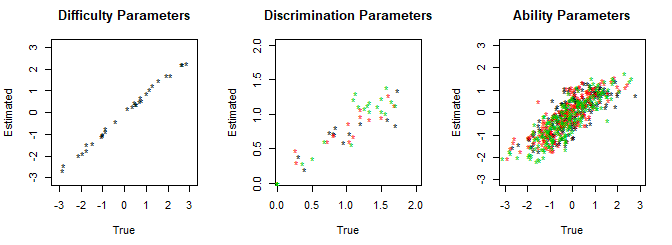
\includegraphics[width=.95\textwidth]{img/ml2pvae_tutorial_plots.png}
  \caption{Correlation plots of IRT parameter estimates produced by the above code tutorial.}
  \label{fig:tutorial_plots}
\end{figure}

\chapter{Details on Related Works}
\sideremark{TODO: remove if I get rid of all related work stuff}


